This chapter presents digitized children's drawings. The first section provides additional context about the art competition, and the following section details the dataset quantitatively. The last section describes the insights obtained through the exploration of drawings and possible directions of studies using this dataset.

\begin{figure}[ht]
\centering
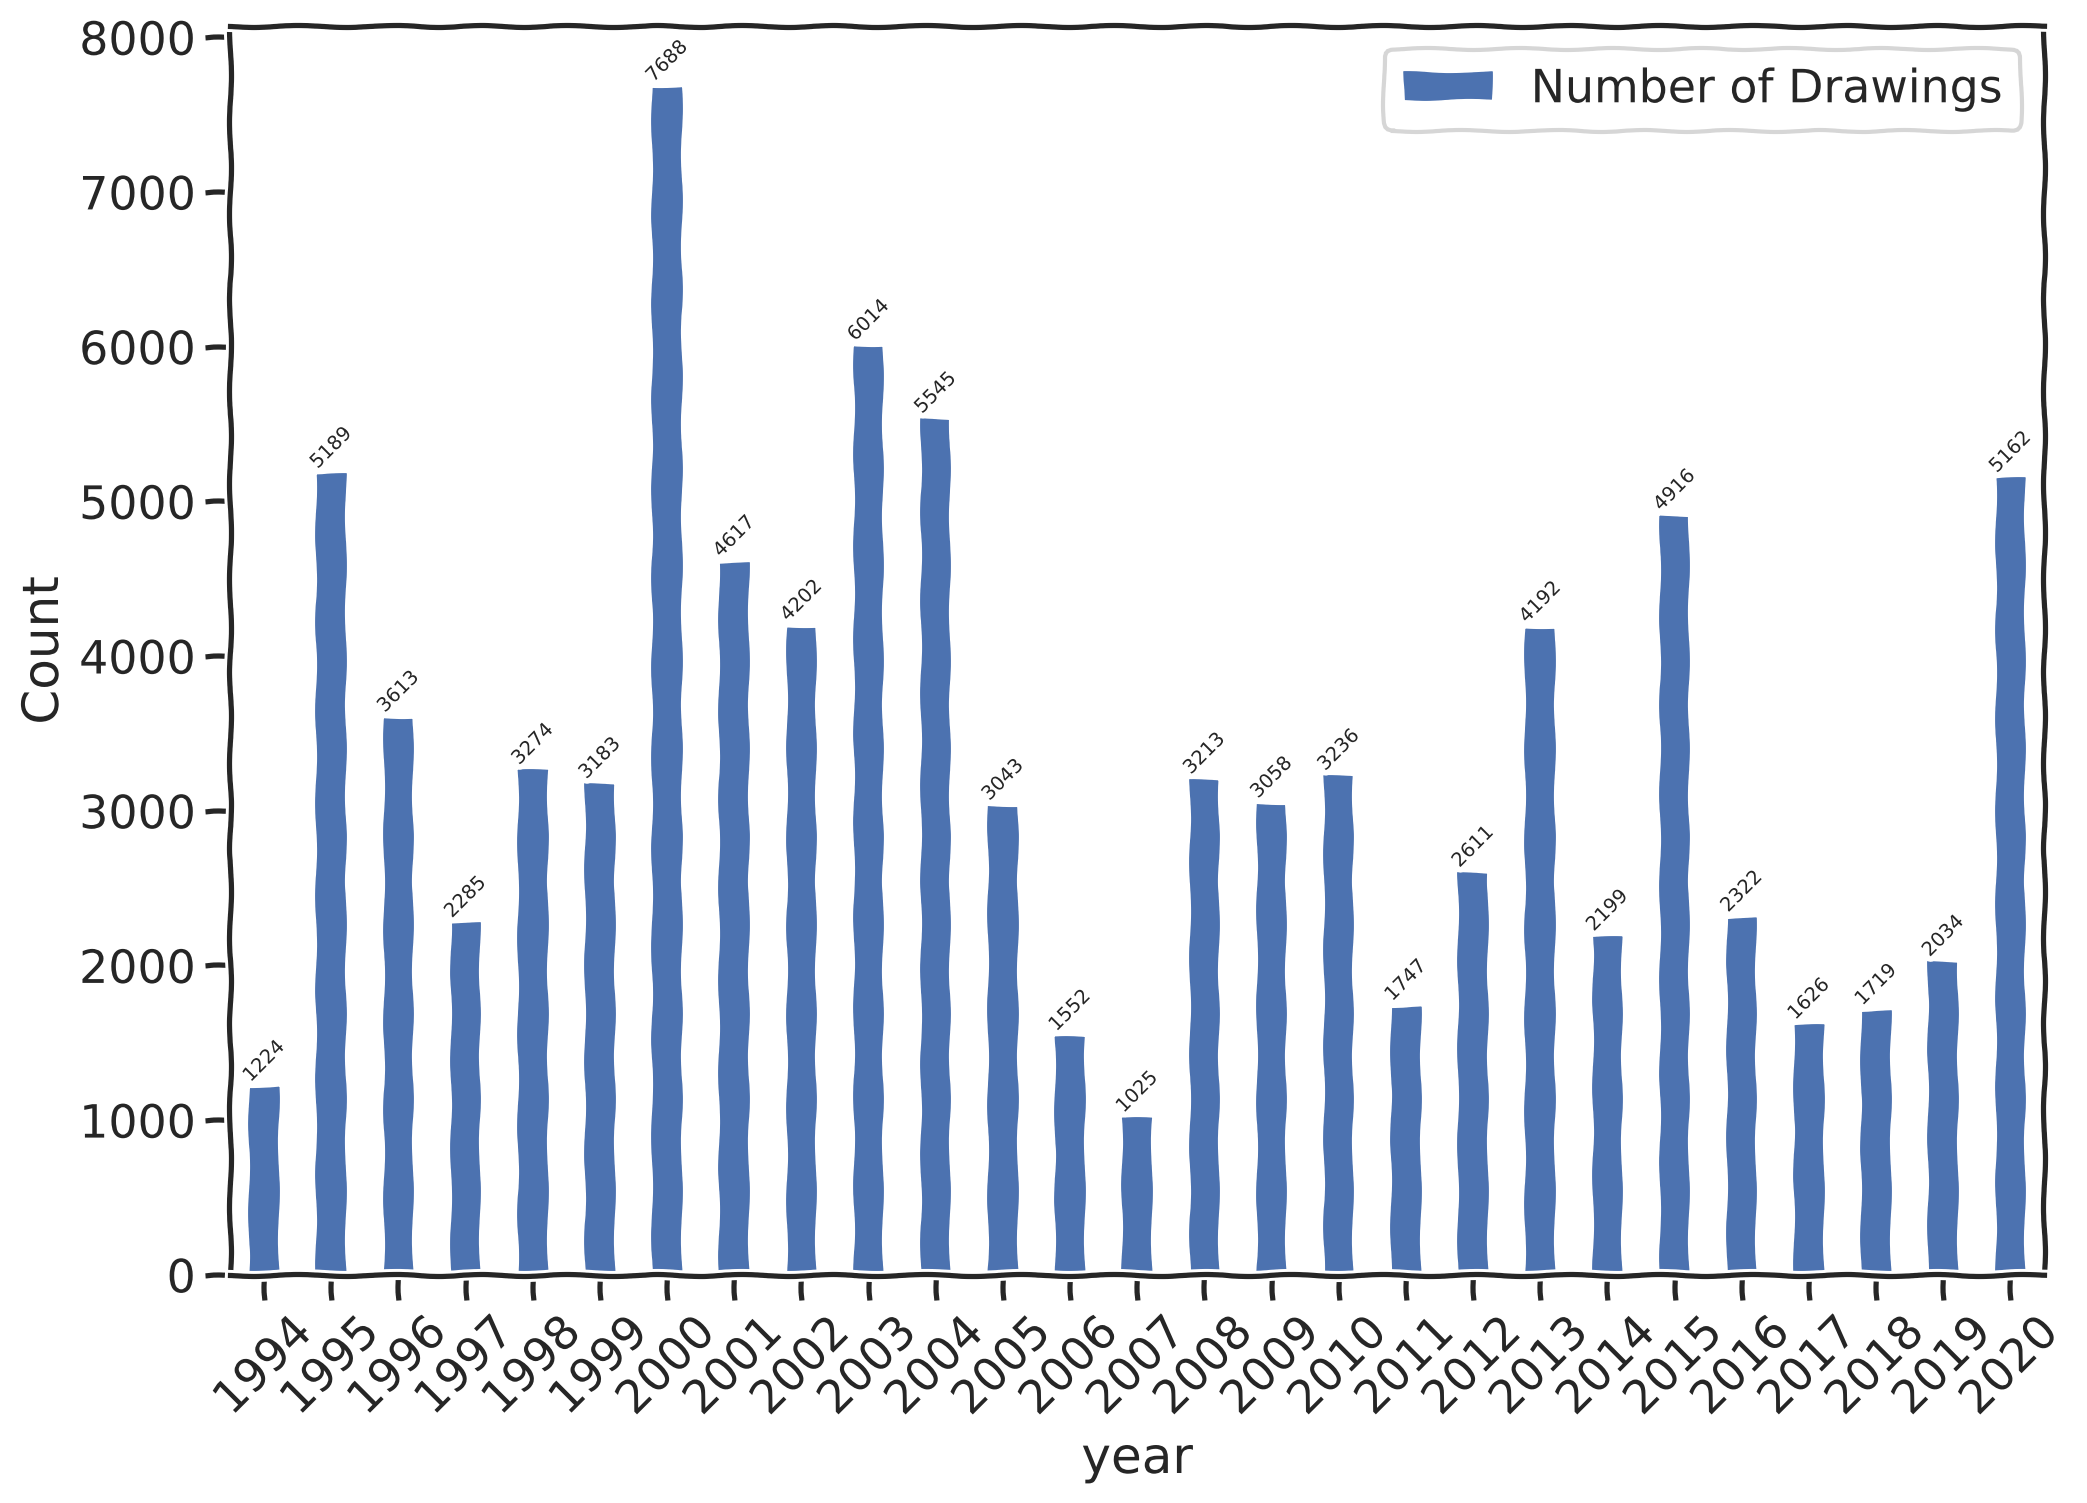
\includegraphics[width=0.96\textwidth]{images/eda_drawings/year_wise_drawings_v2.png}
  \caption{Number of digitized drawings per year}
  \label{fig:drawing-per-year}
\end{figure}

\begin{figure}[ht]
\centering
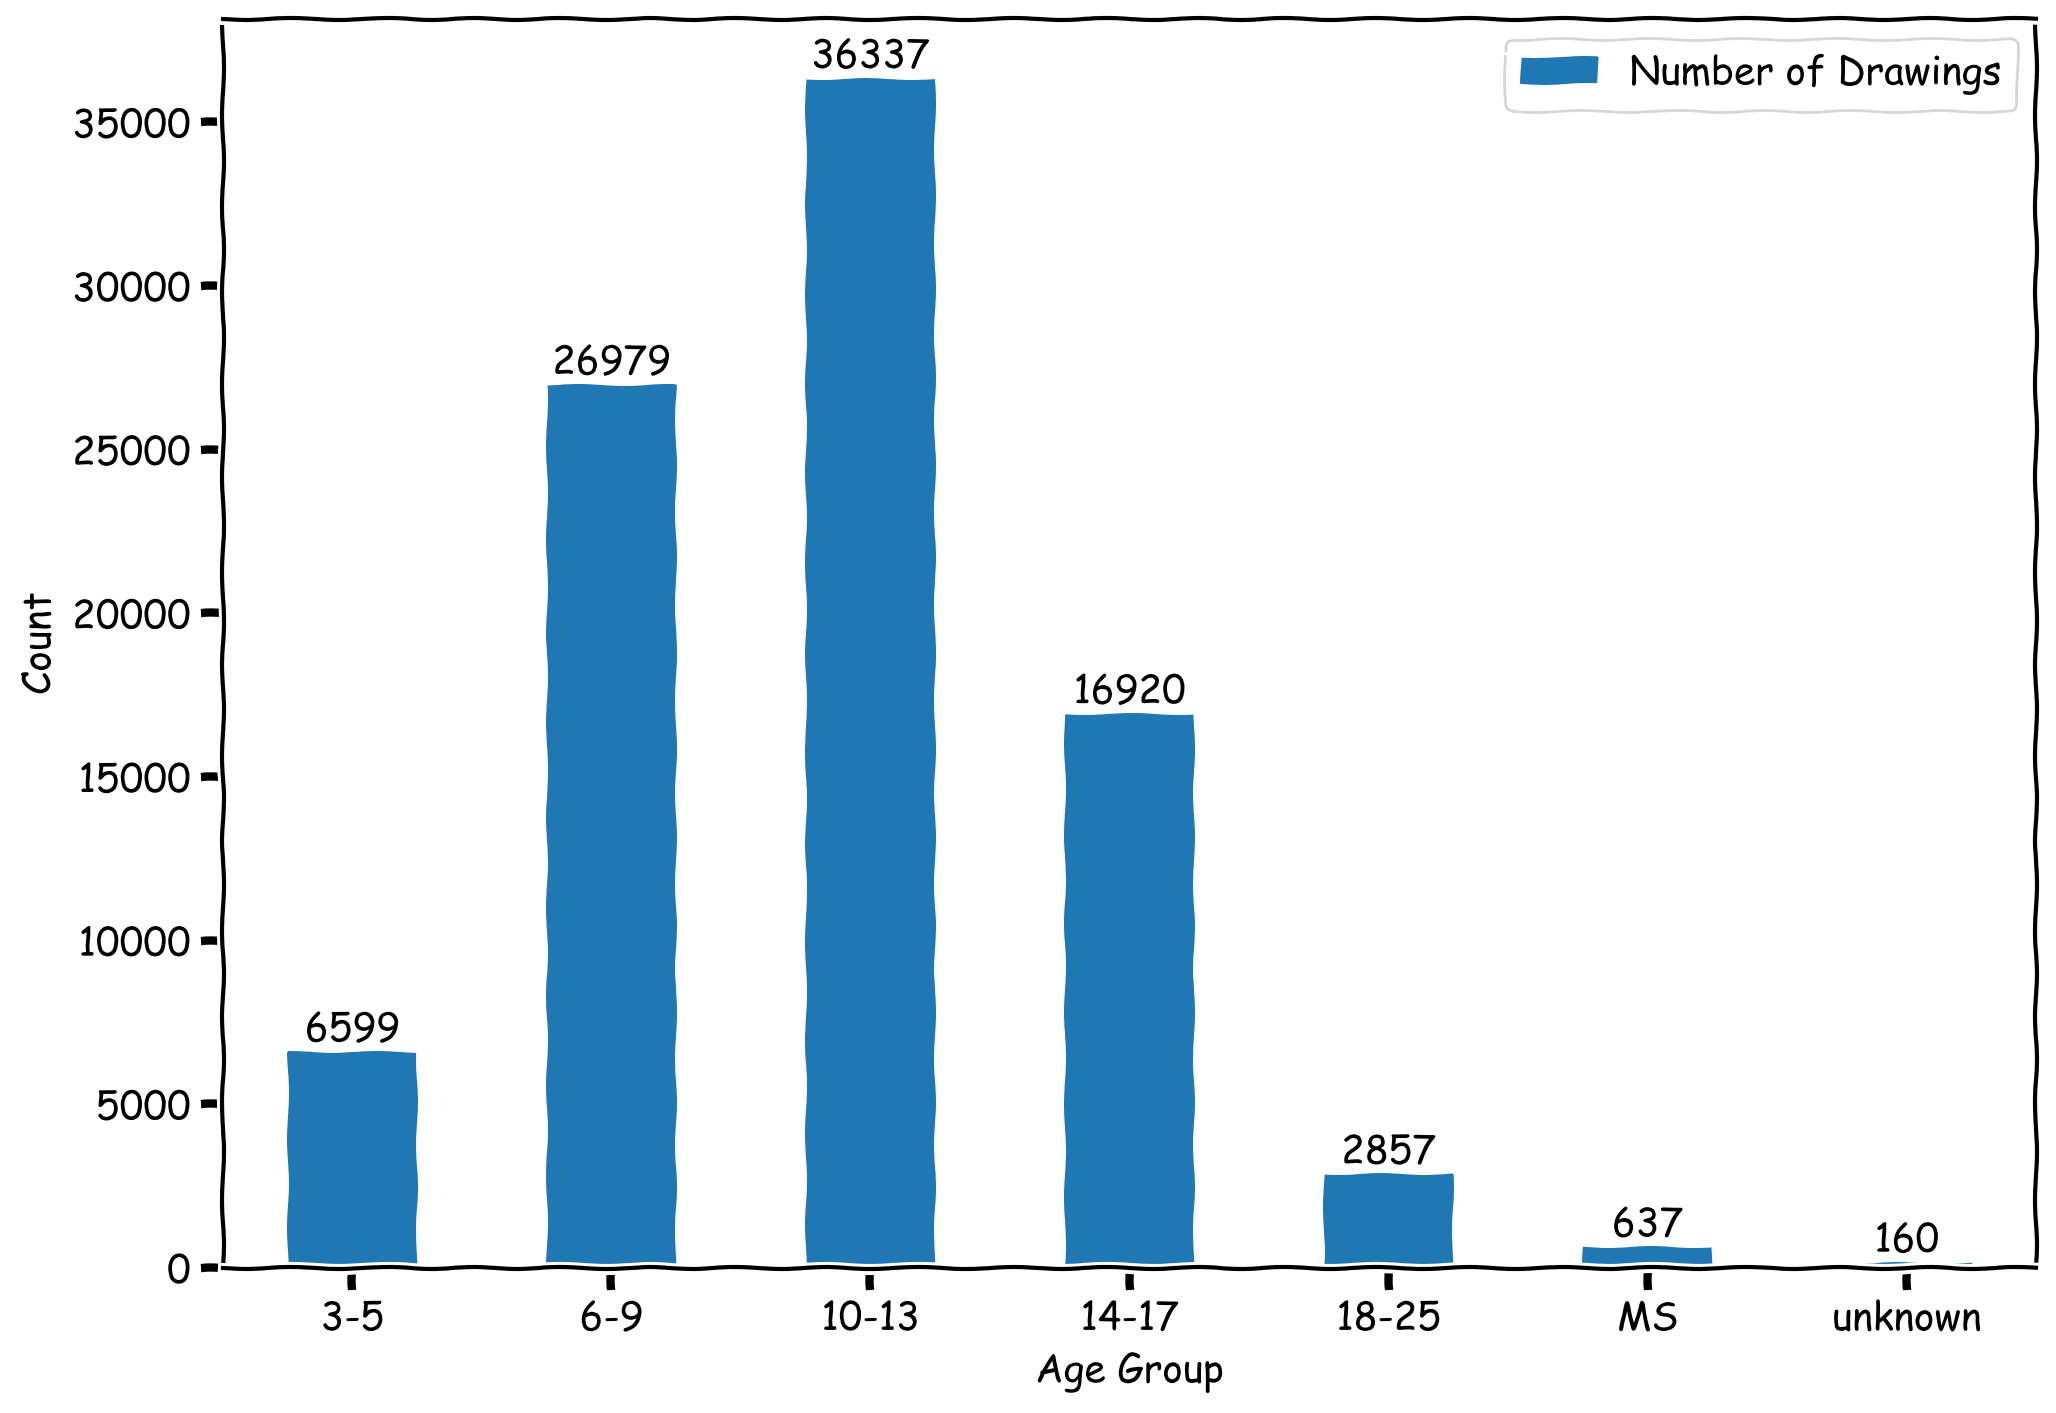
\includegraphics[width=\textwidth]{images/eda_drawings/agegroup_wise_drawings_v2.png}
  \caption{Number of digitized drawings per age group}
  \label{fig:drawing-per-agegroup}
\end{figure}

\begin{figure}[ht]
\centering
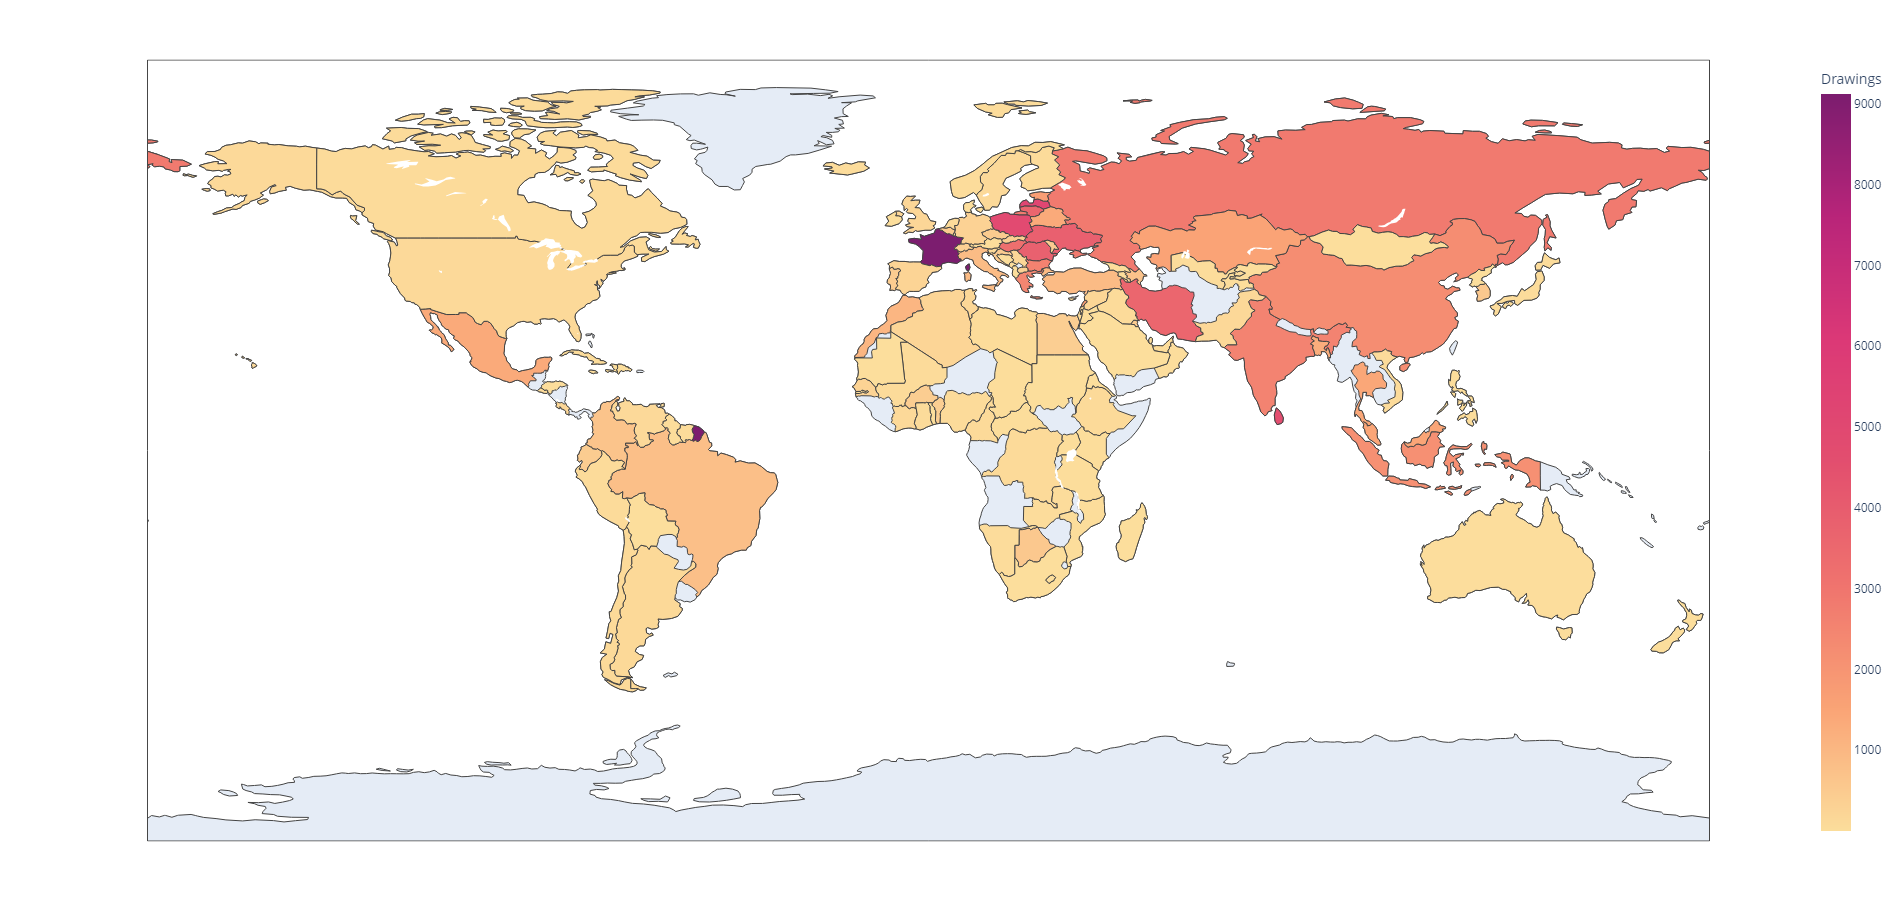
\includegraphics[width=\textwidth]{images/eda_drawings/country_wise_drawings_v1.png}
  \caption{Number of digitized drawings per country}
  \label{fig:drawing-per-country}
\end{figure}

\begin{figure}[ht]
\centering
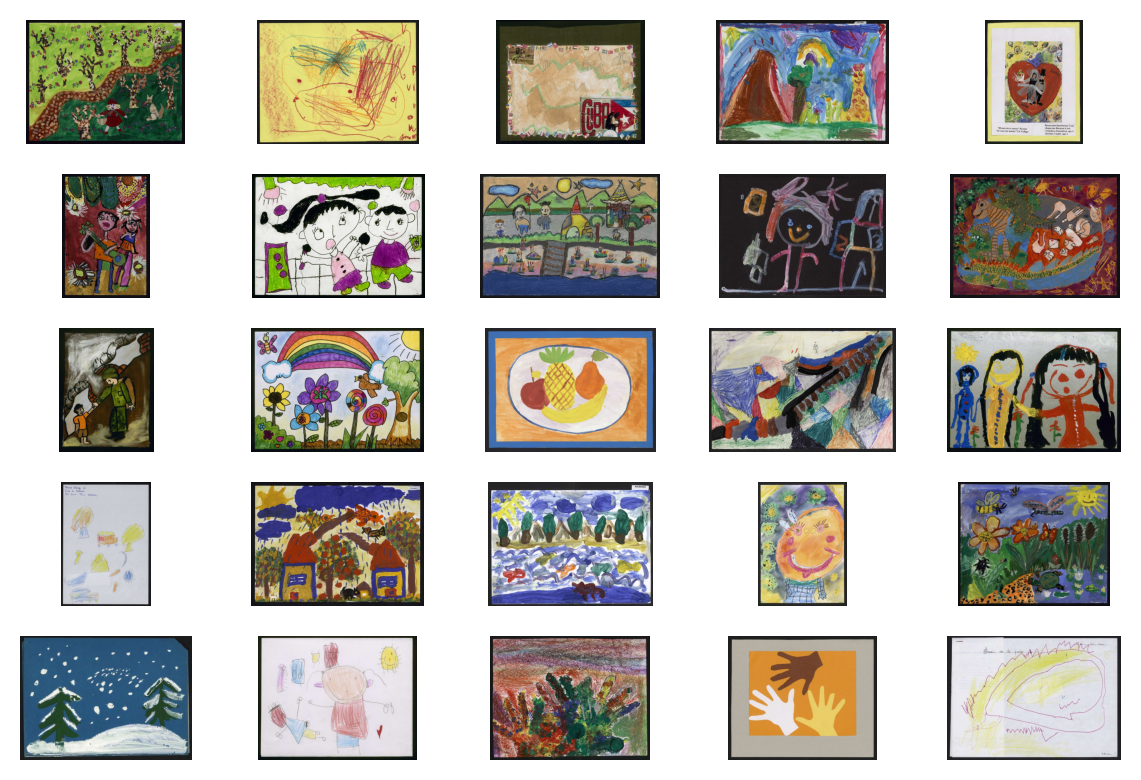
\includegraphics[width=\textwidth]{images/sample_drawings/sample_drawings_3_5.png}
  \caption{Sample drawings by children between 3 to 5 years}
  \label{fig:drawing-3_5}
\end{figure}

\begin{figure}[ht]
\centering
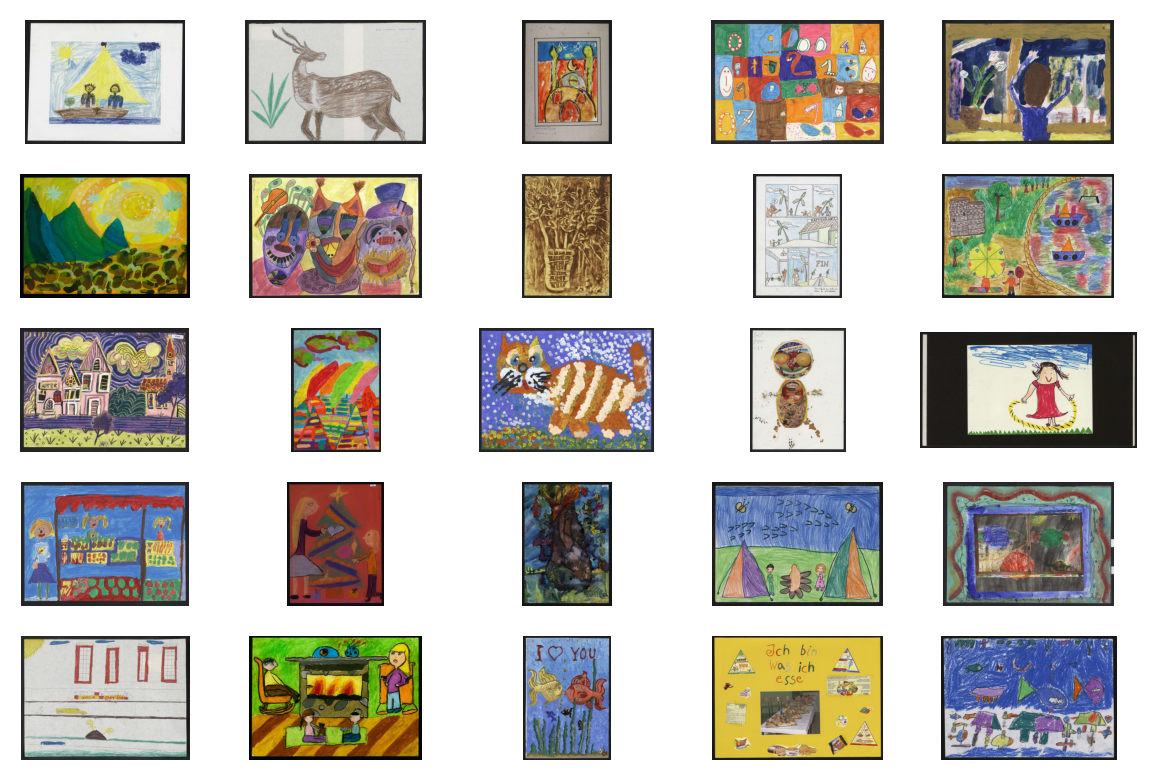
\includegraphics[width=\textwidth]{images/sample_drawings/sample_drawings_6_9.png}
  \caption{Sample drawings by children between 6 to 9 years}
  \label{fig:drawing-6_9}
\end{figure}

\begin{figure}[ht]
\centering
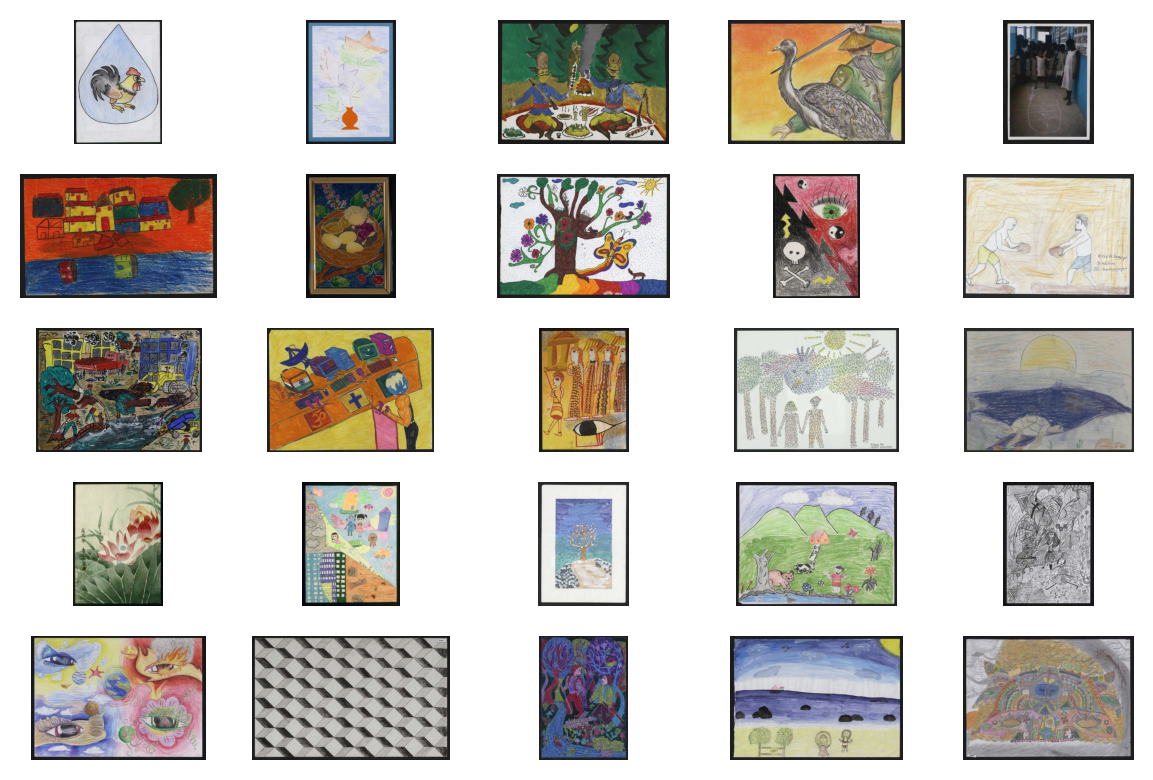
\includegraphics[width=\textwidth]{images/sample_drawings/sample_drawings_10_13.png}
  \caption{Sample drawings by children between 10 to 13 years}
  \label{fig:drawing-10_13}
\end{figure}

\begin{figure}[ht]
\centering
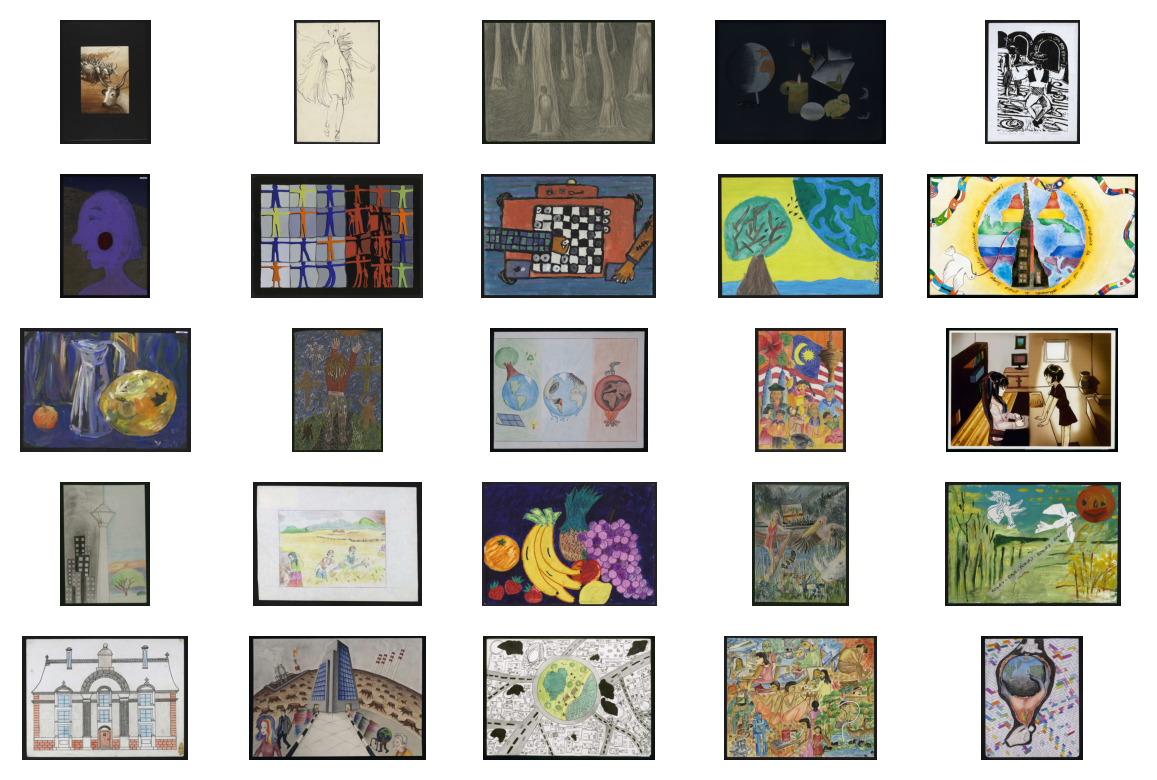
\includegraphics[width=\textwidth]{images/sample_drawings/sample_drawings_14_17.png}
  \caption{Sample drawings by children between 14 to 17 years}
  \label{fig:drawing-14_17}
\end{figure}

\begin{figure}[ht]
\centering
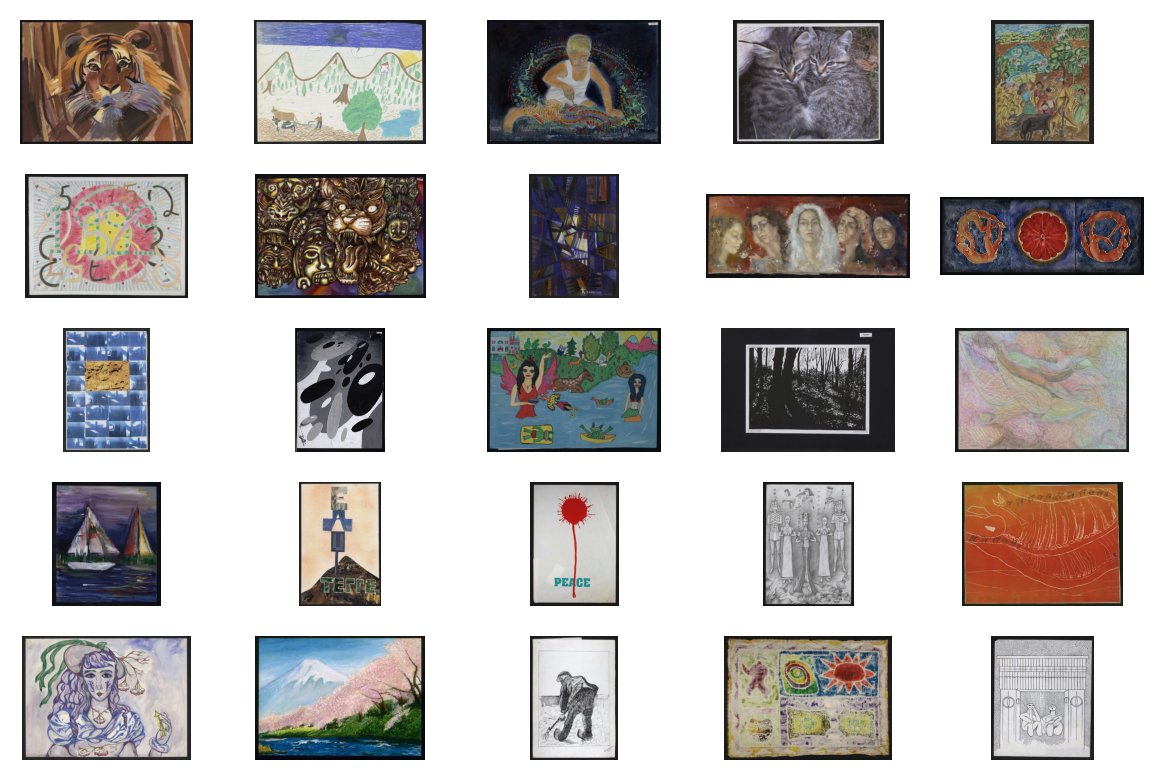
\includegraphics[width=\textwidth]{images/sample_drawings/sample_drawings_18_25.png}
  \caption{Sample drawings by children between 18 to 25 years}
  \label{fig:drawing-18_25}
\end{figure}

\begin{figure}[ht]
\centering
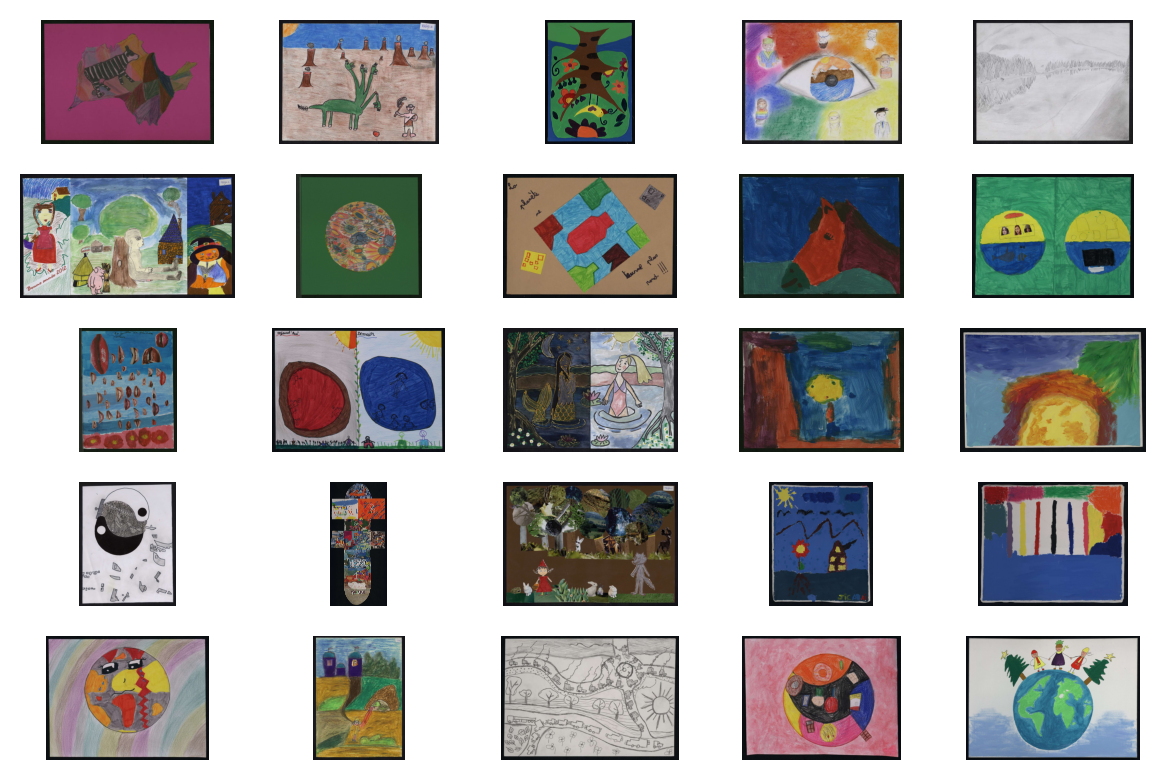
\includegraphics[width=\textwidth]{images/sample_drawings/sample_drawings_MS.png}
  \caption{Sample drawings by children with special medical conditions}
  \label{fig:drawing-MS}
\end{figure}


\section{Graines d’artistes du monde entier}

The \textit{Seeds of artists from around the world} competition provides a space to discuss, deliberate, and develop ideas about the happening issues of this world. The \emph{Institut Mondial d'Art de la Jeunesse} or \textit{World Youth Art Institute} (IMAJ, in short) selects a topic that challenges the planet as a theme and centers the competition around that theme. IMAJ conducts the competition in collaboration with more than 1000 institutions from 150 countries around the world. As mentioned previously, IMAJ continues to preserve more than 100,000 submissions they received since the competition's inception at the \textit{Mémoires du Futur}. To further preserve the multi-dimensional diverse cultural heritage, IMAJ initiated the digitization process of the drawings collection in 2017, and more than 90,000 works are already digitized. Besides conservation, other digitization objectives include allowing digital consultation, facilitating research, and enabling analysis using computational tools of the collection \cite{centre_unesco_2020}.


\section{Digitized Drawings Dataset}

Any submission to the art competition has at least two sides, the illustration on the front and some metadata on the back. The metadata of each drawing is almost always handwritten and very few times in print. At the time of writing this thesis, 179,427 scans (including the front and the back) were available, and nearly 90,000 contained an illustration\footnote{The number of drawings is not exactly half of the scans because some of them had more than one front side}. The drawings are categorized based on young artists' country and age group. The file name of the scan, made up of six parts, provides this information. The six parts are the year of submission, age group, unique id, country of origin, side of the scan, and the quality of the scan (high-quality scan for archiving and standard quality for consultation).

Elemental analysis of this metadata reveals that the collection has 26 years of drawings from 1994 to 2020 (including both years). Also, there are six age groups: 3-5, 6-9, 10-13, 14-17, 18-25, and Medico-Social (MS) for children with special needs. On average, 3352 drawings are available per year, with a significant hike in a few years, and Figure \ref{fig:drawing-per-year} shows their spread over the years\footnote{As some of the drawings are yet to be available in digital format, it is too early to remark on the low number of drawings in specific years.}. Figure \ref{fig:drawing-per-agegroup} shows the drawings available per age category, and they predominantly belong to the 10-13 (40\%), 6-9 (30\%), and 14-17 (18\%) groups. Table \ref{tab:year-age-distribution} shows drawings distribution per year across each age category. Lastly, Figure \ref{fig:drawing-per-country} shows the drawings per country on a map. France is the highest contributor with 10\% (9120), followed by Latvia (5.7\%), Poland (5.4\%), Sri Lanka (5.1\%), and Ukraine (4.2\%) in the top five. The age and country are not available in the filename for nearly 985 drawings. Figures \ref{fig:drawing-3_5} - \ref{fig:drawing-MS} show the sample drawings from 6 different age categories.

\section{Insights and Research Directions}\label{chap:3:sec:research-dir}
Before zeroing on the current research question, the drawing collection was explored manually. While the rest of the thesis discusses identifying drawings similar to well-known artworks, this section summarizes the insights obtained during the exploration and provides directions for further research.

Every year, the children base their illustrations on the theme provided by the IMAJ, producing a diverse set of drawings that vary in technique and substance. The techniques include crayons, pencil sketching, watercolours, gauche, pastels, acrylic, ballpoint pen, ink, photos, and computer graphics. Parallelly, the children use a diverse set of styles, Fauvist, Cubist, Surrealist, Figurative, Hyperrealist, and Abstract, to name a few. Unsurprisingly, the drawings of children under five are primarily scribbles and re-creation of common subjects around them like houses, rivers, and mountains. This novelty steadily changes through the ages of 6 to 18, and substantial new creations appear in older individuals. A clear distinction exists between the works of young artists based on their country in terms of style. Nonetheless, the references in the drawings cross the nation's borders, and the artistic response to international issues is at the same level as domestic ones.


\subsection{Metadata Extraction}
The metadata about the artist and the school is available on the verso (back) side of the drawing. With some minor differences, overall, the drawings contain the metadata detailed below. However, only the age and country information was extracted during the digitization process and stored in the file name. 
\begin{itemize}
	\item About the Artist
		\begin{itemize}
			\item Name
			\item Address
			\item Phone number
			\item Birthday/Age
			\item Sex
			\item Disability status
		\end{itemize}
	\item About the Drawing
		\begin{itemize}
			\item Title/Description
			\item Technique
			\item Size
		\end{itemize}
	\item About the institution
		\begin{itemize}
			\item Name of the institute
			\item Address of the institute
			\item Name of the teacher/professor
		\end{itemize}
\end{itemize}
Extracting this multi-lingual data that is partially handwritten and partially in print is challenging. At the same time, this metadata offers an opportunity to identify the artists and schools and analyze the works at a more granular level. In addition, this metadata will aid the ongoing efforts at the IMAJ to create a web platform to access the collection. Lastly, the description of the work by the young artists themselves gives a clear and unfiltered explanation of their work and helps us understand their interpretation of the theme.

\subsection{Iconographic analysis}
The influence of culture, especially the traditions at various levels, is clearly reflected in the drawings. These ideas are represented as subjects or background objects or through colors. For example, religious symbols such as \textit{Stupas} or Christian art often appear in drawings from some regions. Some works commonly contain animals and houses. These icons appear irrespective of the themes, and a correlation between age and place of origin was observed. In line with the current work, deep learning models can help in detecting and localizing icons in the drawings. Exploring this treasure of iconography aids in understanding the evolution of their usage, tracing the circulation of symbols in drawings, and the social patterns they reveal. 

\subsection{Realization of themes by young minds}
Although each child receives an identical description of the competition theme, their realization of it as a drawing differs from one another. Each one uses backgrounds, elements, and objects differently from the others. Extracting the information about these entities present in the drawings across countries, age groups, and themes and looking through the historic date calendar provides an opportunity to understand the effect of socio-economic and political events on the children. It could also unearth classic cross-cultural references used to represent the same or similar ideas by children across the globe.

\subsection{Clustering and artistic signatures}
For some years, the themes of the competition were repeated with a different title, and most submissions were through art schools or institutions. These two factors might have influenced the children to reuse patterns, and ideas, improve existing work, or work together with a friend. In fact, some drawings are complete only when combined with others. This last direction of work proposes to group the creations by the children that share a visual and thematic similarity separately and together. This investigation can help declutter up to what extent the drawings from an institute are homogenous and the tendency to repeat patterns.